\section{Automatic Differentiation}

In order to obtain the required derivatives for the optimization process of a PINN, one could either resort to manually obtaining them and coding them, or numerically with a method such as central differences or symbolically where a program can manipulate expressions and provide a closed-form of the required function. ~\cite{Automatic}

All methods mentioned above are unsuitable for deep-learning applications .

Manual differentiation is very error prone, if not humanly-impossible for very deep nets.
Numerical differentiations of the form

\begin{align}
  \frac{\partial f(\mathbf{x})}{\partial x_i} \approx \frac{f(\mathbf{x} + h\mathbf{e}))}{h}
\end{align}

is easy to implement, but round-off and truncation errors make it unacceptable for the gradients of deep-learning problems, which can be dependent on millions of parameters.

Symbolic differentiation, addresses the issues of manual and numerical differentiation, but its expression can be complex and suffer from "expression swell", the time required to compute a derivative scales together with the complexity of the expression.

Automatic Differentiation (also known as \emph{algorithmic differentiation}) can tackle effectively the aforementioned issues.
Automatic Differentiation relies on the chain rule $(f \circ g)' = (f'\circ g)\cdot g'$consists of two modes, \emph{forward accumulation} and \emph{backward accumulation}, which dictate how one can reach $dy/dw_i$ from $dw_i/dx$ and vice versa.

\begin{figure}[!ht]
  \centering
  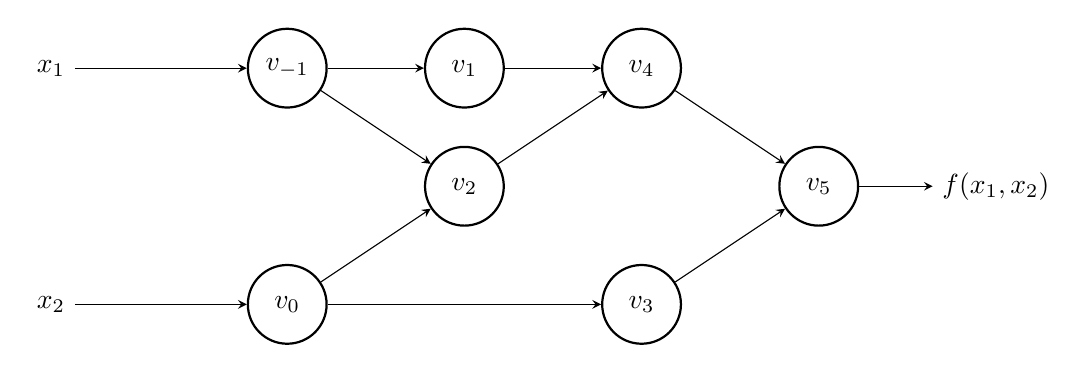
\begin{tikzpicture}[x=1.5cm, y=1.0cm, >=stealth]
\begin{scope}[]
    \node (x1) at (-2,1.5) {$x_1$};
    \node (x2) at (-2,-1.5) {$x_2$};
    \node (f) at (6,0) {$f(x_1, x_2)$} ;
\end{scope}

\begin{scope}[every node/.style={circle,thick,draw, minimum size=1cm}]
    \node (v-1) at (0,1.5)  {$v_{-1}$};
    \node (v1)  at (1.5,1.5)  {$v_1$};
    \node (v4)  at (3,1.5) {$v_4$};
    \node (v2)  at (1.5,0) {$v_2$};
    \node (v5)  at (4.5,0) {$v_5$};
    \node (v0)  at (0,-1.5) {$v_0$};
    \node (v3)  at (3,-1.5) {$v_3$};
\end{scope}

\begin{scope}[ ]
    \path [->] (x1) edge (v-1);
    \path [->] (v-1) edge (v1);
    \path [->] (v-1) edge (v2);
    \path [->] (v1) edge (v4);
    \path [->] (v2) edge (v4);
    \path [->] (v4) edge (v5);
    \path [->] (x2) edge (v0);
    \path [->] (v0) edge (v3);
    \path [->] (v0) edge (v2);
    \path [->] (v3) edge (v5);
    \path [->] (v5) edge (f);
\end{scope}
\end{tikzpicture}

  \caption{"The forward accumulation graph"}
\end{figure}
